\section{Introducing Queues}
\label{sec:introducing_queues}


\begin{frame}
	\frametitle{Stuck in traffic}

	\begin{center}
		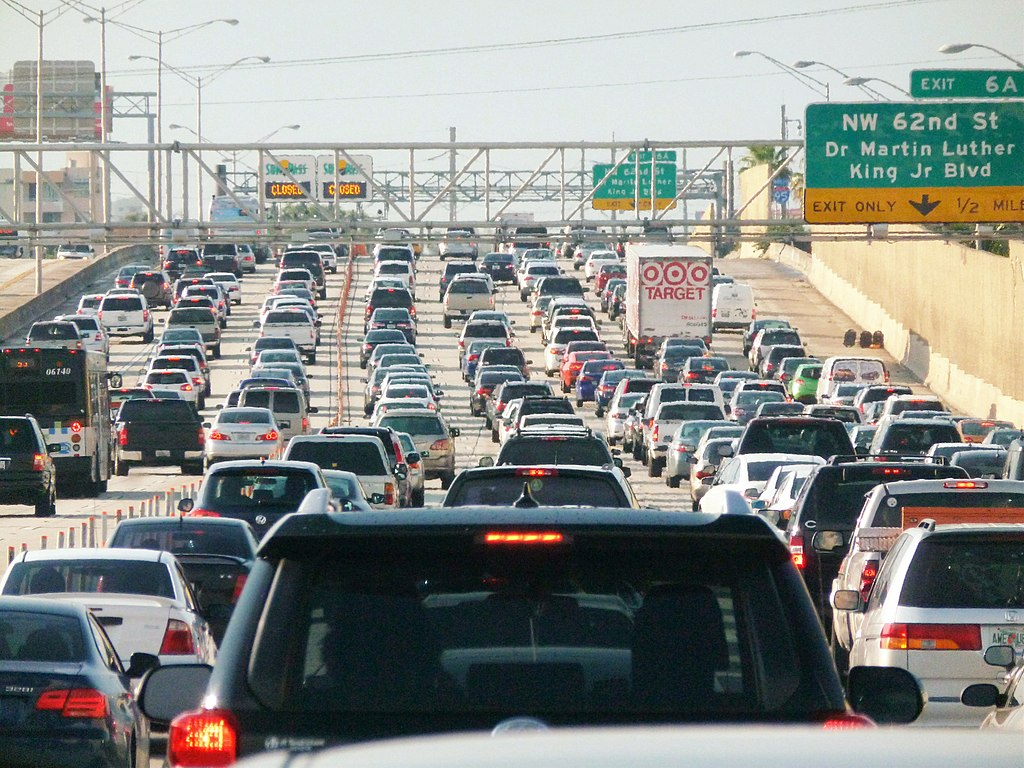
\includegraphics[width=0.5\textwidth]{figures/traffic.jpg}\\
		\hspace*{15pt}\hbox{\scriptsize Image By:\thinspace{\itshape B137}}
	\end{center}
	% https://commons.wikimedia.org/wiki/File:Miami_traffic_jam,_I-95_North_rush_hour.jpg
\end{frame}

\begin{frame}
	\frametitle{Me and my books}
	\framesubtitle{A life-long story cont'd}

	\begin{columns}
		\column{0.455\textwidth}
			\begin{center}
				\alt<4->{
					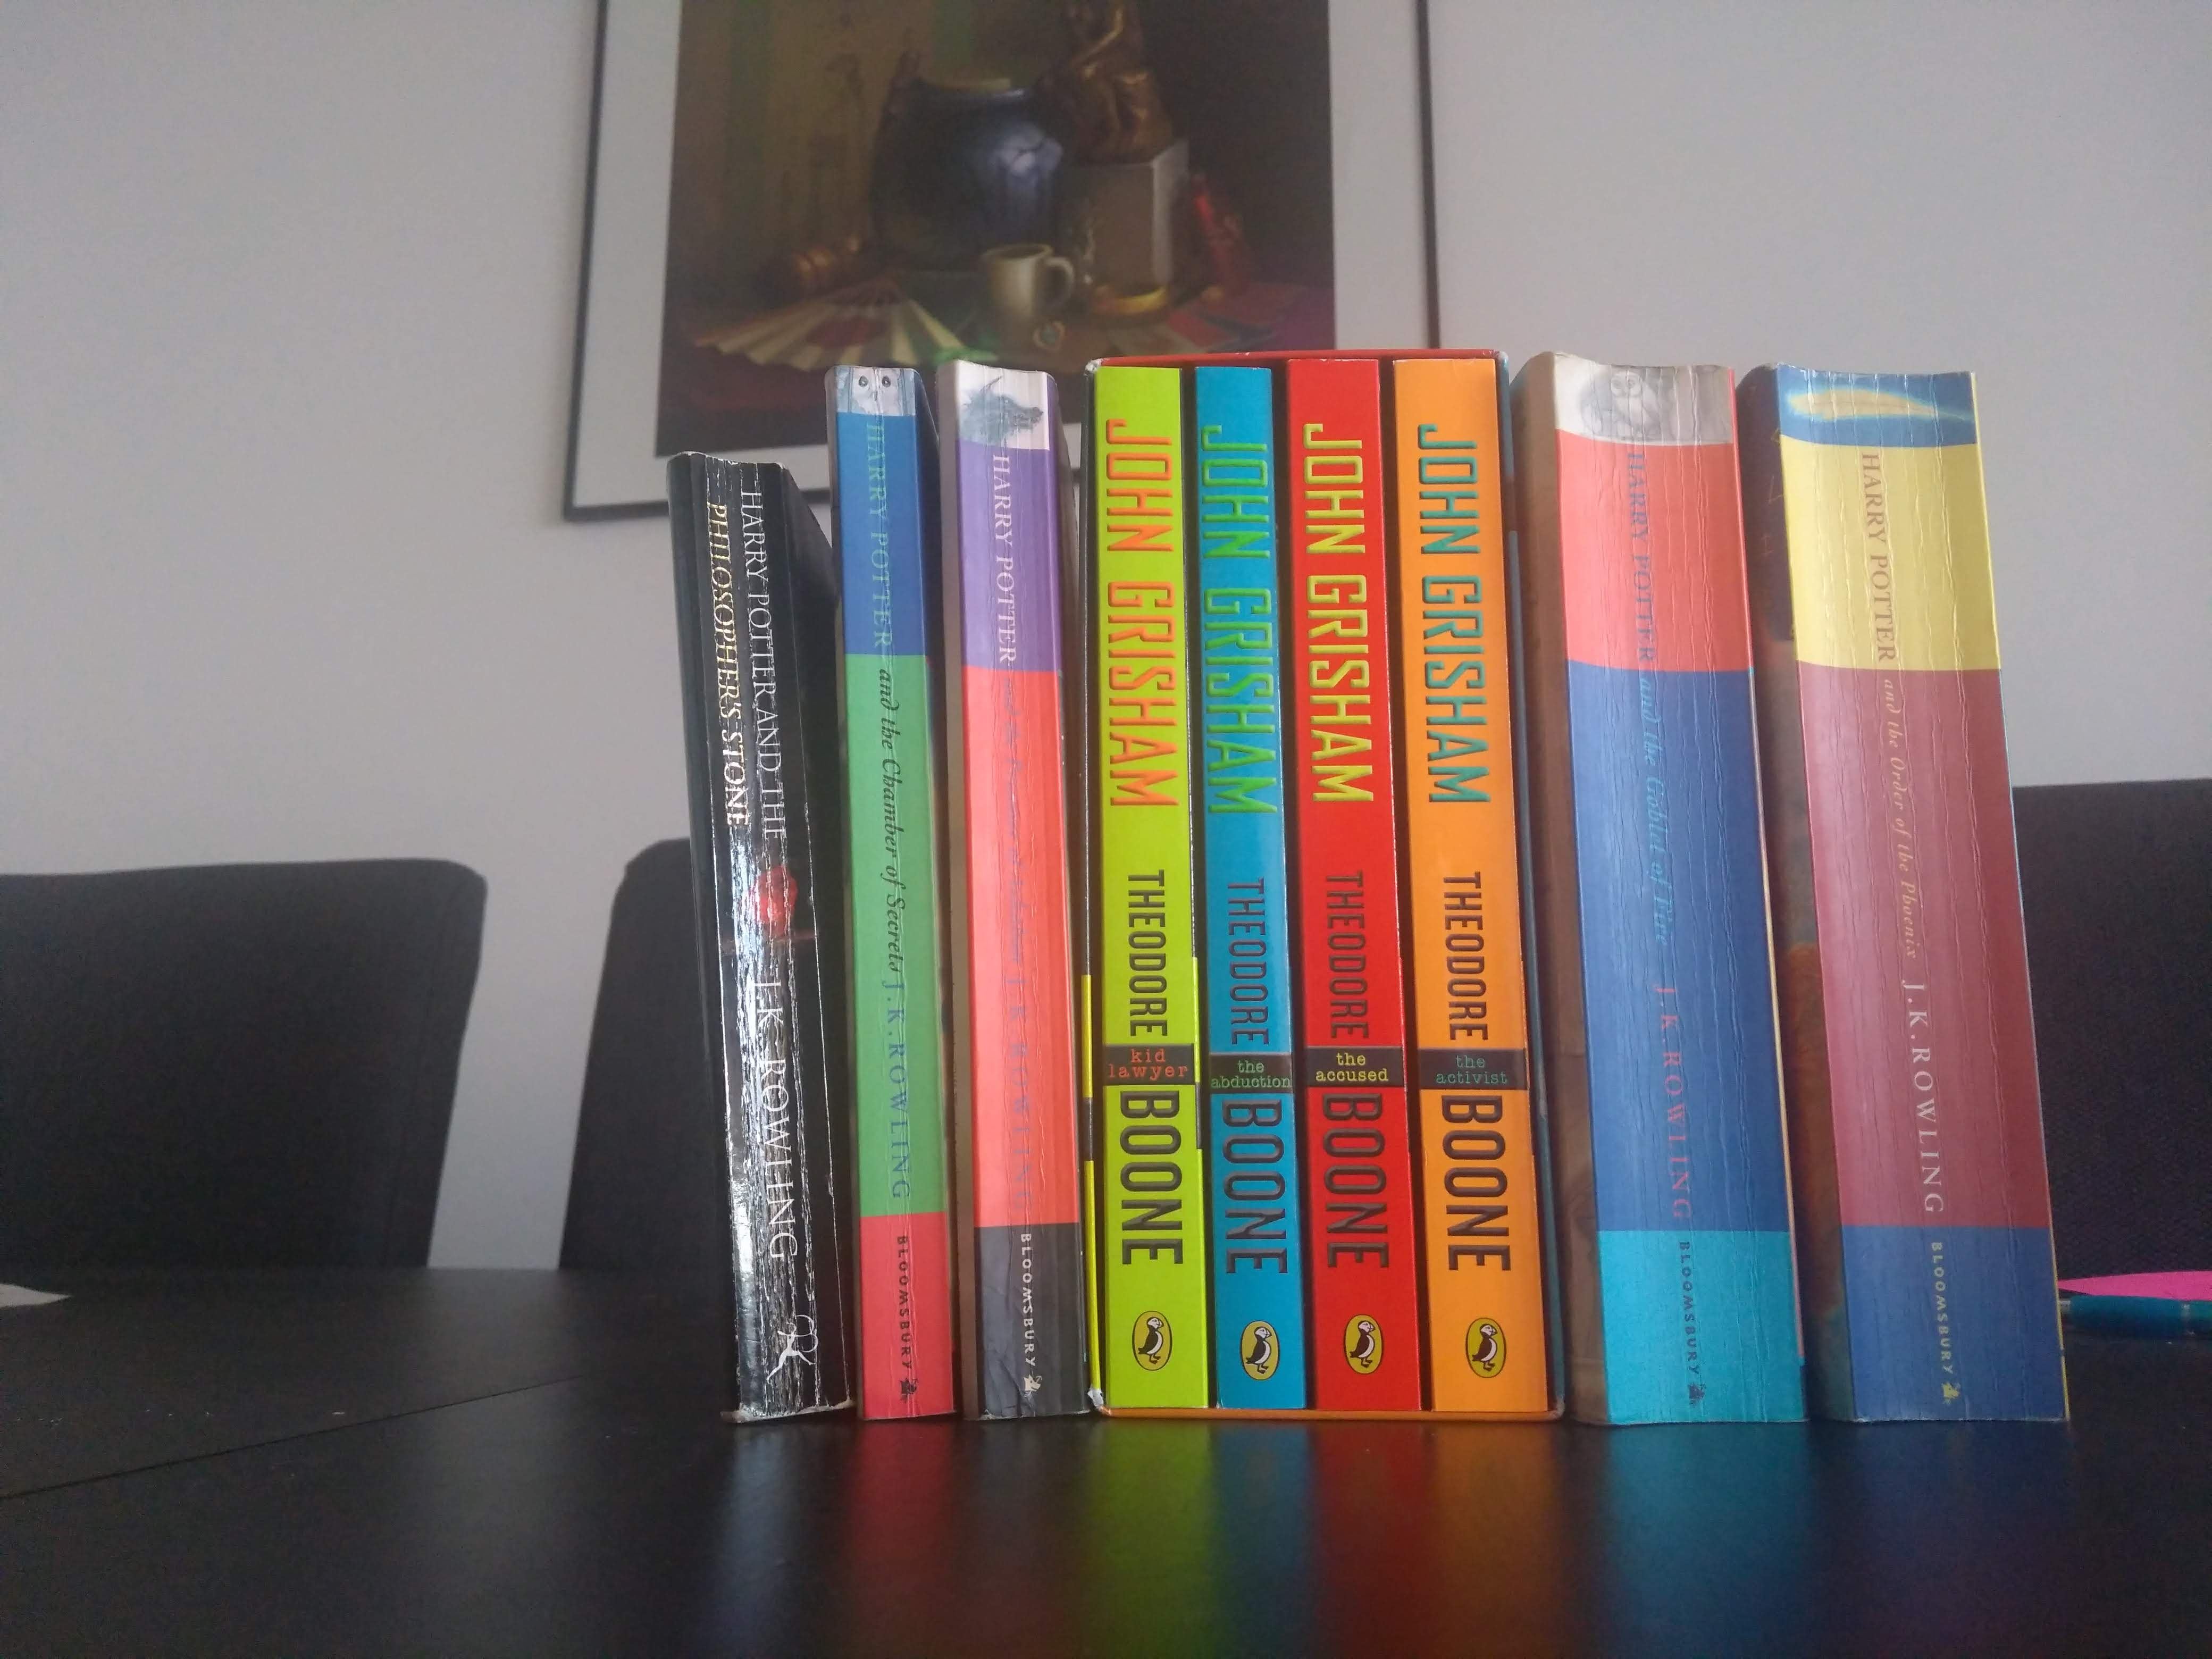
\includegraphics[width=\textwidth]{figures/queue_read.jpg}\\
					}{
					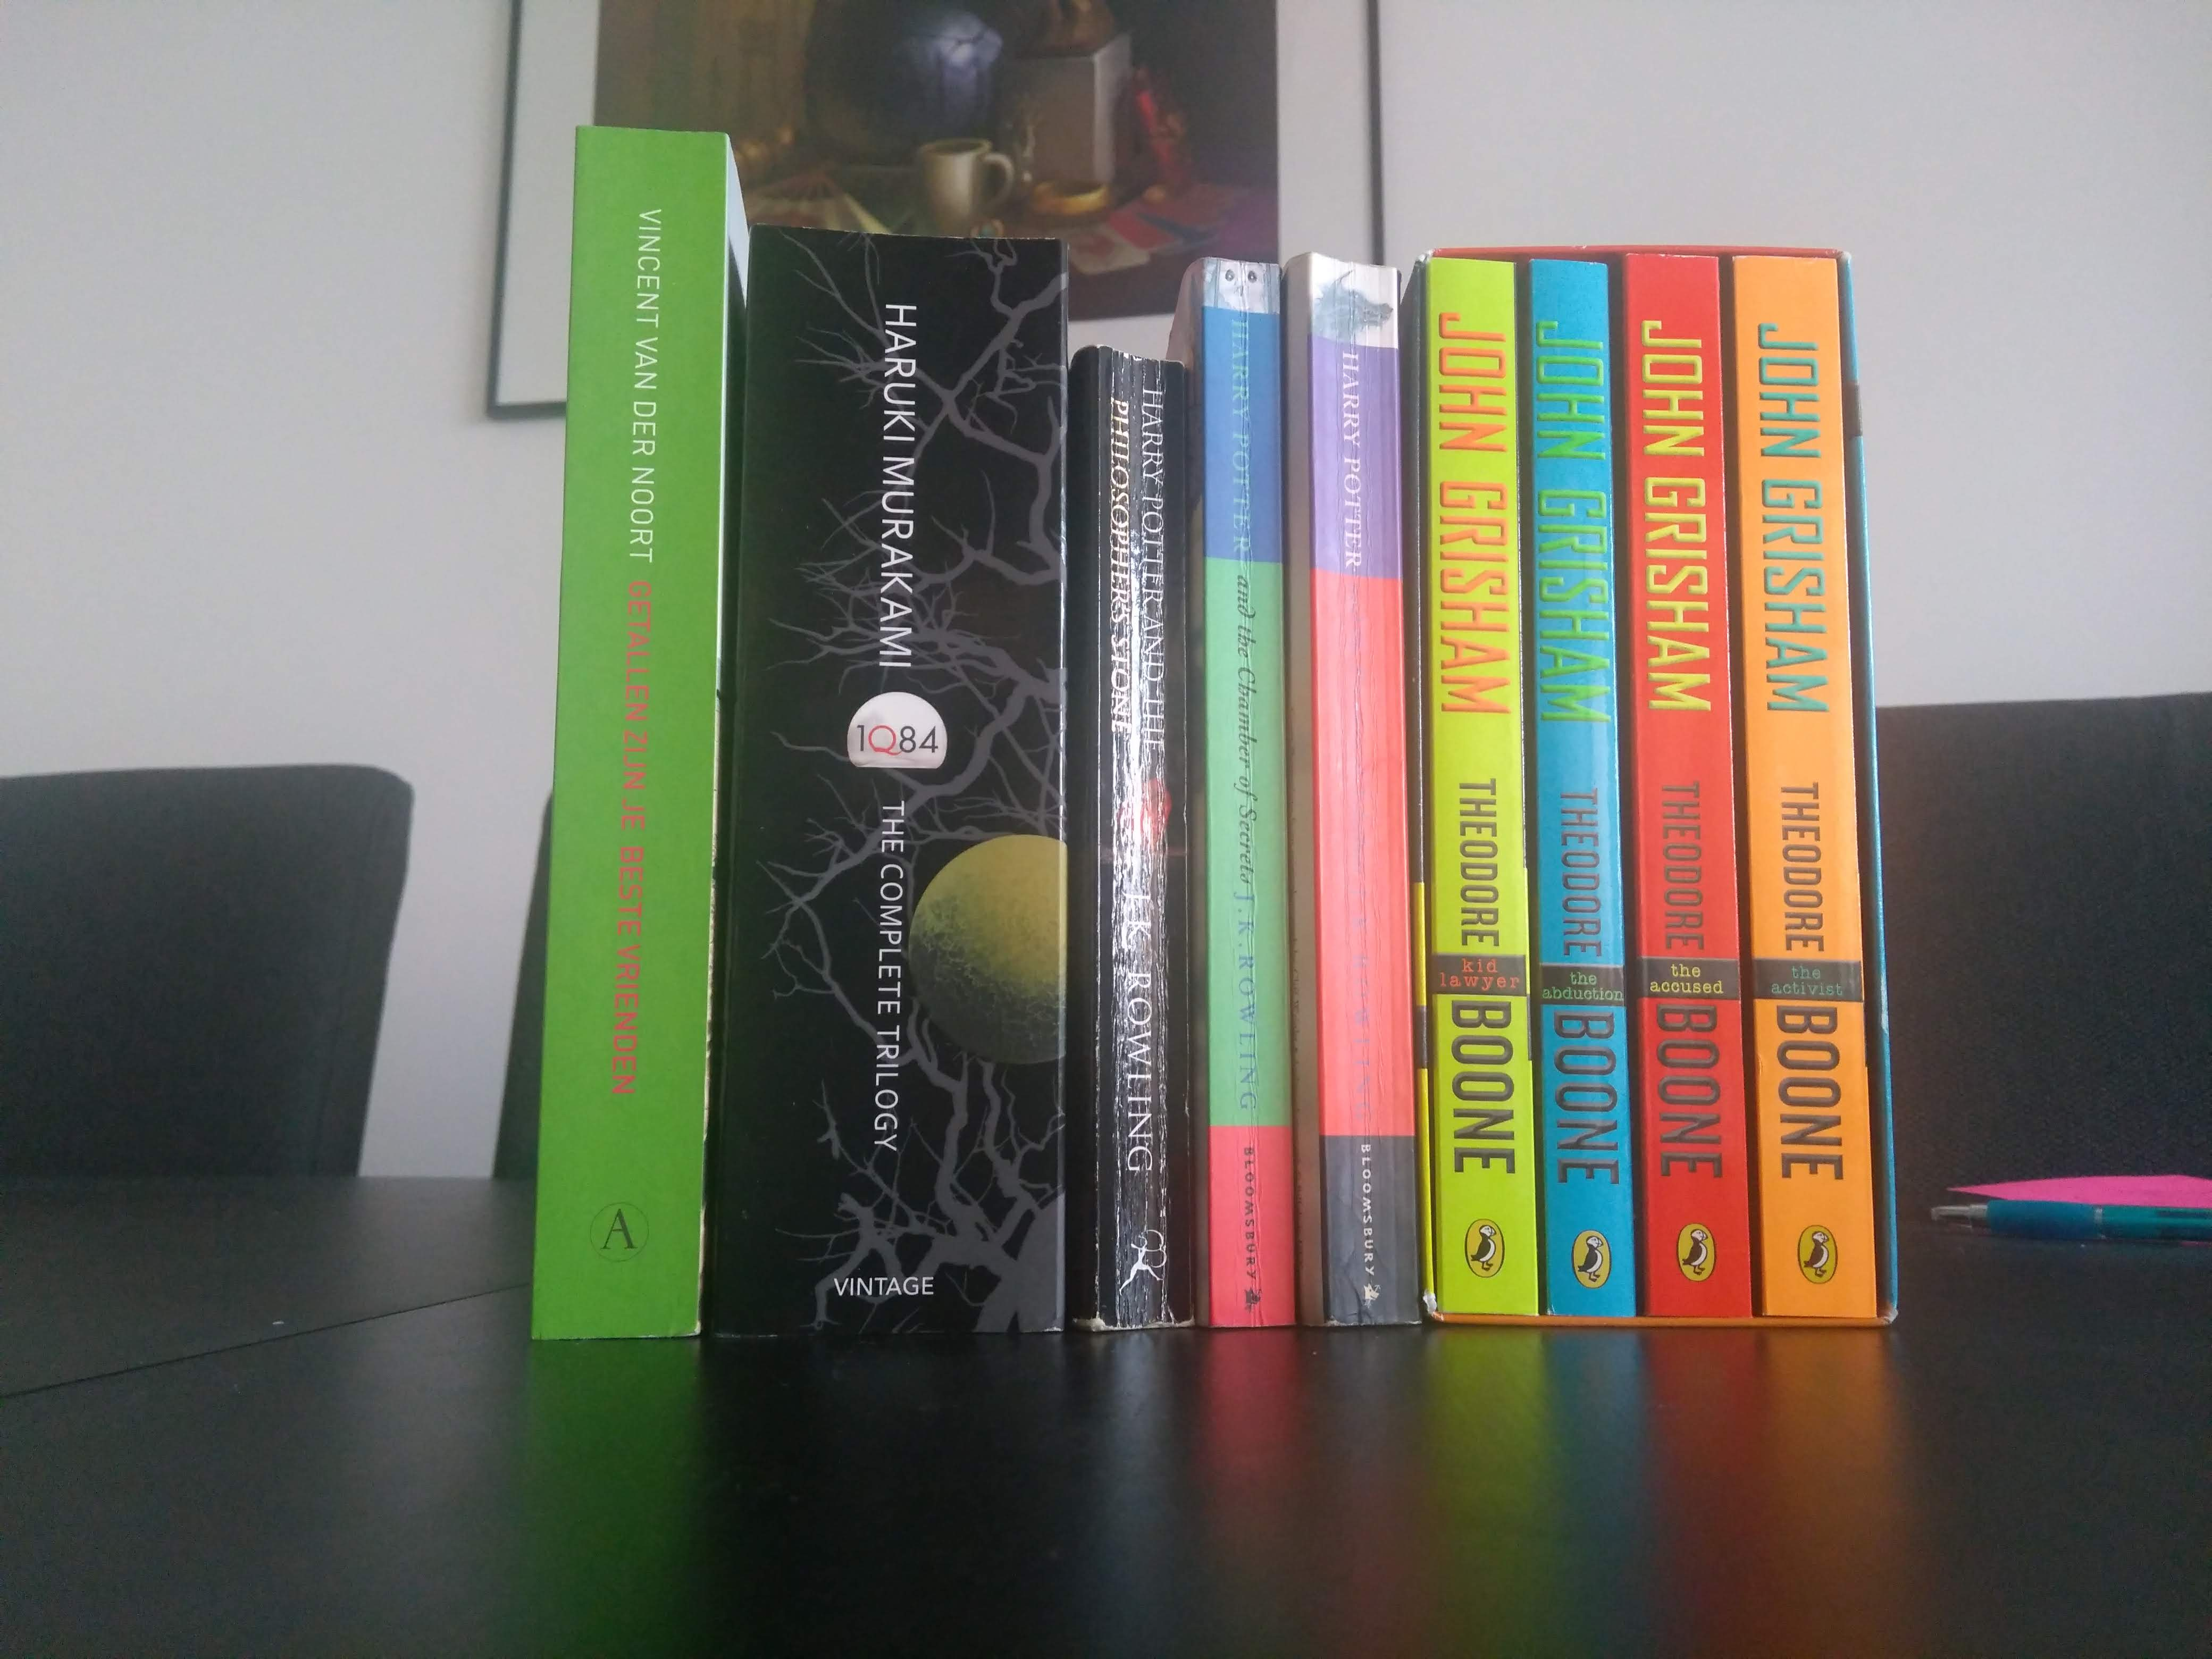
\includegraphics[width=\textwidth]{figures/queue_unread.jpg}\\
					}
				\hspace*{15pt}\hbox{\scriptsize Image By:\thinspace{\itshape Stefan Hugtenburg}}
				\hspace*{15pt}\hbox{\scriptsize Bookcovers and picture in the back by others}
			\end{center}
		\column{0.455\textwidth}
		\begin{itemize}
			\item This is how I now store books I still want to read.
				\pause
			\item A nice \alert{queue} of books, with new ones going on the right.
				\pause
			\item After finishing one, I take the next one from the left
				\pause
			\item So after a few weeks\dots
				\pause
			\item This uses the \alert{FIFO}-principle.
		\end{itemize}
	\end{columns}
\end{frame}

\begin{frame}
	\frametitle{The what!?}
	\framesubtitle{FIFO}
	
		\begin{block}{FIFO}
			The \textit{First-In-First-Out}, or FIFO, principle is the working of a queue.\\
			\pause
			The first thing we've added to the queue is the first thing we take out.\\
			\pause
			Similarly the last we have added to the queue, is the last to be taken out.
		\end{block}	
\end{frame}

